\documentclass[11pt]{article}
\usepackage{fullpage,amsthm,amsfonts,amssymb,epsfig,amsmath,times,algorithm,algorithmic}
\usepackage[table,xcdraw]{xcolor}

\newtheoremstyle{indented-remark}
{}
{}
{\addtolength{\leftskip}{2.5em}}
{}
{\bfseries}
{:}
{.5em}
{}

\newtheoremstyle{indented-proof}
{}
{}
{\addtolength{\leftskip}{2.5em}}
{}
{\slshape}
{.}
{.5em}
{}

\theoremstyle{definition}
\newtheorem{theorem}{Theorem}
\newtheorem{lemma}{Lemma}
\newtheorem{corollary}{Corollary}
\newtheorem{observation}{Observation}
\newtheorem{definition}{Definition}

\theoremstyle{plain}
\newtheorem{claim}{Claim}

\theoremstyle{indented-remark}
\newtheorem{case}{Case}

\theoremstyle{indented-proof}
\newtheorem*{proofofcase}{Proof of Case}

\begin{document}

\begin{center}
{\bf\Large CMPS 102 --- Fall 2018 ---  Homework 1}
\end{center}

\begin{center}
\textit{"I have read and agree to the collaboration policy." - \textbf{Kevin Wang}}
\end{center}

\section*{Solution to Problem 4: Perfectly Imperfect Masterpieces}

Given Bob's specifications, we want to write an algorithm that helps him design the alignment of the L-shaped blocks for any square with length $2^n$ units, where $n \in \mathbb{N}$. The black 1 unit square shown in Figure 0 is a blank spot on the masterpiece.

\centerline{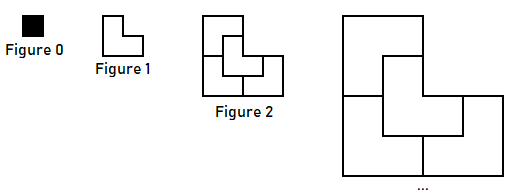
\includegraphics[scale=1]{images/fig3.png}}

\begin{algorithm}
\caption{Recursively creates a perfect imperfect masterpiece for any $n$.}
\begin{algorithmic} 
\STATE \textbf{PERFECT-IMPERFECT} ($n$):
\STATE Initialize a blank masterpiece $M$
\STATE Initialize $L$ as the L-shaped block shown in Figure 1.
\STATE \textit{FILL-MP} ($M, L, n$)
\STATE 
\STATE \textbf{FILL-MP} ($M, L', n$):
\IF{$n = 0$}
\STATE Add the imperfection shown in Figure 0 to the top right corner of $M$
\ELSE[$n > 0$]
\STATE Add the segment $L'$ to the bottom left of $M$
\STATE Let $L'$ be the augmented segment created with 4 of itself as shown in Figure 2.
\STATE \textit{FILL-MP} ($M, L', n - 1$)
\ENDIF
\end{algorithmic}
\end{algorithm}

\begin{claim}
The algorithm is correct for all $n \in \mathbb{N}$.
\end{claim}

\begin{proof}
Let $P(n)$ be the statement: "The algorithm designs a perfect imperfect masterpiece for a square of size $2^n$". \newline

\noindent The base cases of $P(0)$ and $P(1)$ are true.

\centerline{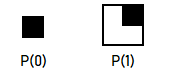
\includegraphics[scale=1]{images/fig4.png}}

\noindent Assume for a square with side $2^n$, where $n > n_{0}$ and $n_{0} = 1$, that $P(n)$ is true. We need to prove that $P(n + 1)$ is true. \newline

\noindent Let a square with side of $2^{n + 1}$ be equivalent to a square with side $2^n$ in quadrant I, in addition to the $L'$ segment that fills quadrants II, III, and IV. 

\centerline{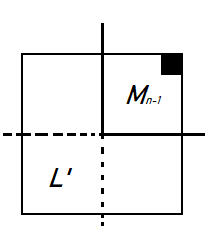
\includegraphics[scale=1]{images/fig5.png}}

\noindent Using the induction hypothesis, we assume that the square in quadrant I is a correctly designed masterpiece. The additional $L'$ segment is formed solely of nested $L'$ segments of smaller size. Thus, the final square maintains the properties that define a perfect imperfect masterpiece. Thus $P(n) \implies P(n + 1)$ is true, proving that the algorithm will design a correct masterpiece.
\end{proof}

\noindent The run time of adding a block $L$ to a masterpiece takes $O(1)$. When creating the augmented $L'$ segment, it takes four individual $L'$ segment placements. The recursion is run a total of $n$ times. Thus, a total of $4^n$ L-shaped blocks are placed. The time complexity of this algorithm is: $O(2^{2n})$.

\end{document}